\chapter{Rust}

\section{安装和配置}
默认情况下,Rust及其工具集Cargo都会被安装到/root/.rust和/root/.cargo,或者
是C:$\backslash\backslash$Users$\backslash\backslash$zhangjl$\backslash\backslash$AppData下,
只针对当前用户有效。有的时候,我们需要针对所有用户有效,因此,需要更改安装
路径。Rust提供了2个环境变量,进行安装路径的修改,其使用如下:
\begin{code-block}{bash}
export CARGO_HOME=/opt/cargo
export RUSTUP_HOME=/opt/rustup
export PATH=/opt/cargo/bin:$PATH
\end{code-block}

Windows,则是修改系统的环境变量,将CARGO\_HOME和RUSTUP\_HOME指向合适的
位置即可。然后再执行安装程序即可(windows执行可执行程序):
\begin{code-block}{bash}
curl --proto '=https' --tlsv1.2 -sSf https://sh.rustup.rs | sh
\end{code-block}

安装完毕之后,通常需要进行一些安装和配置,方便其他的代码编辑器可以使用代码
补全。操作如下(Linux/Windows通用):
\begin{code-block}{bash}
rustup toolchain add nightly
rustup component add rust-src rls rust-analysis
cargo +nightly install racer
\end{code-block}

如果需要对Rust和相关的工具进行升级,则操作如下:
\begin{code-block}{bash}
rustup update
cargo +nightly install racer
\end{code-block}

\section{Rust的交叉编译}
Rust本身也支持进行交叉编译,可以在Linux下完成针对ARM/Windows的目标文件的编译。
默认情况下,Rust的工具链只会包含当前操作系统默认支持的工具链。查看工具链可
如下操作:
\begin{code-block}{bash}
rustup target list
\end{code-block}

其结果大致如下图\nameref{fig:rust_target}所示。
\begin{figure}[H]
  \centering
  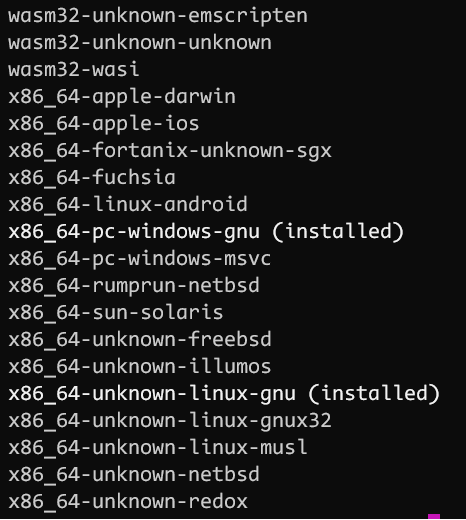
\includegraphics[scale=0.5]{rust_target.png}
  \caption{Rust支持的目标文件架构}
  \label{fig:rust_target}
\end{figure}

需要编译对应架构的目标文件,则需要添加对应架构的工具链
\begin{code-block}{bash}
# 针对ARM V7架构的工具链
rustup target add armv7-unknown-linux-gnueabihf
# 针对ARM X64架构的工具链
rustup target add aarch64-unknown-linux-gnu
# 针对Windows 64的工具链
rustup target add x86_64-pc-windows-gnu
\end{code-block}

除了添加工具链之外,还需要安装对应的交叉编译工具
\begin{code-block}{bash}
# 针对Windows 64的交叉编译工具
dnf install mingw64-gcc mingw64-winpthreads-static -y
\end{code-block}

而针对ARM V7以及ARM X64的交叉编译工具,则是使用gcc-linaro工具链即可。

针对Windows 64的交叉编译方法比较简单,其编译指令如下:
\begin{code-block}{bash}
cargo build --release --target=x86_64-pc-windows-gnu
\end{code-block}

针对ARM V7和ARM X64的编译过程稍微复杂一些,以ARM V7为例,其操作如下:
\begin{enumerate}
  \item 创建配置文件:进入rust工程的根目录
\begin{mdframed}[topline=false, bottomline=false, leftline=false, rightline=false, backgroundcolor=lbcolor]
\begin{minted}[fontsize=\scriptsize,linenos=false,breaklines=true,breakanywhere,breaksymbolleft=,breakanywheresymbolpre=,]{bash}
mkdir .cargo
touch .cargo/config
\end{minted}
\end{mdframed}

  \item 修改配置文件,设置交叉编译工具
\begin{mdframed}[topline=false, bottomline=false, leftline=false, rightline=false, backgroundcolor=lbcolor]
\begin{minted}[fontsize=\scriptsize,linenos=false,breaklines=true,breakanywhere,breaksymbolleft=,breakanywheresymbolpre=,]{bash}
cat >.cargo/config<<EOF
[target.armv7-unknown-linux-gnueabihf]
linker = "/opt/gcc-linaro-7.5.0-2019.12-x86_64_arm-linux-gnueabihf/bin/arm-linux-gnueabihf-gcc"
ar = "/opt/gcc-linaro-7.5.0-2019.12-x86_64_arm-linux-gnueabihf/bin/arm-linux-gnueabihf-ar"
EOF
\end{minted}
\end{mdframed}

  \item 进行交叉编译:
\begin{mdframed}[topline=false, bottomline=false, leftline=false, rightline=false, backgroundcolor=lbcolor]
\begin{minted}[fontsize=\scriptsize,linenos=false,breaklines=true,breakanywhere,breaksymbolleft=,breakanywheresymbolpre=,]{bash}
cargo build --release --target=armv7-unknown-linux-gnueabihf
\end{minted}
\end{mdframed}

\end{enumerate}
